\chapter{面向天基协同计算的区块链平台架构与设计}

在前文中，本文围绕天基网络协同计算卸载问题，分别从系统建模、系统层协同优化以及任务层实时决策三个层面展开研究。第2章建立了面向天基协同计算的系统模型，明确了节点异构、链路时变、任务随机到达以及多主体协作等关键特征；第3章提出了基于区块链与多智能体强化学习的系统层协同资源分配方法，从全局层面实现可信状态共享与协同优化；第4章进一步提出了基于联邦学习与深度强化学习的任务层并发感知卸载方法，实现面向局部任务到达场景的实时决策。至此，全文已经形成"系统层全局协同—任务层局部决策"的双层智能管控框架。

然而，前述研究主要集中于模型构建与算法设计层面。若缺乏统一的平台承载机制，第3章提出的系统层协同优化方法与第4章提出的任务层卸载决策方法仍难以在真实分布式环境中形成稳定、可信且持续演化的运行体系。一方面，系统层协同优化依赖跨节点可信状态同步与一致性规则支撑；另一方面，任务层实时决策依赖模型版本治理、执行结果回流和行为存证机制。若仍采用传统集中控制方式或松散耦合式系统拼接方式，则难以同时满足状态可信、规则可执行、行为可追溯和跨层可协同等要求。

基于此，本章在第2章系统建模结果以及第3章、第4章算法设计的基础上，提出一种面向天基协同计算的区块链平台架构。该平台并非将区块链作为附加的安全模块，而是将其作为连接系统层资源协同与任务层实时卸载的分布式可信底座，通过轻量级联盟链共识、分层链结构、链上/链下协同机制以及智能合约治理体系，实现关键状态共享、任务行为存证、模型版本溯源与执行反馈闭环。

本章围绕平台设计动机与总体思路、总体架构与分层链设计、区块结构与数据流转机制、双层智能方法的平台映射与运行闭环，以及工程可行性分析等五个方面展开。其目的不是在前文之外再增加一个独立模块，而是依托已完成的平台项目，将第2章系统建模、第3章系统层协同资源分配方法与第4章任务层并发感知卸载方法统一映射到一个可运行、可验证、可审计的平台环境中。

\section{平台设计动机与总体思路}

\textbf{平台设计动因。}
天基协同计算卸载问题本质上并非单一任务的转发或调度问题，而是在动态网络条件下，由多类异构节点共同参与的状态感知、资源竞争、任务迁移、行为反馈与规则治理问题。尤其在本文所研究的场景中，卫星节点既可能作为任务发起方，也可能作为协同计算资源提供方，节点之间在共享资源与竞争收益的同时，还受到拓扑时变、链路波动和任务突发到达等多种不确定因素影响。这决定了仅依靠单节点局部决策或单次优化求解，难以从根本上解决天基环境下的持续协同问题。

第3章从系统层角度出发，构建了基于区块链与多智能体强化学习的协同资源分配方法，重点解决多节点在全局资源竞争背景下如何实现状态可信共享与协同策略学习。然而，该方法成立的前提在于系统中存在一个可为多主体提供统一规则约束和可信共享信息的支撑环境。若节点之间缺乏一致的状态同步与审计机制，则系统层智能体获取的全局状态可能受局部偏差或虚假上报影响，从而削弱系统层协同优化的有效性。

第4章从任务层角度出发，提出了基于联邦学习与深度强化学习的并发感知卸载方法，解决任务到达瞬间如何在局部环境下做出实时卸载决策的问题。该方法在运行过程中需要依赖联邦学习模型的持续更新、模型参数的一致性校验、任务执行结果的回流反馈以及跨节点行为的可追溯记录。若缺乏统一平台，任务层方法虽然可以在局部条件下形成决策，但其模型版本治理、执行结果可验证性以及长期策略迭代能力将难以保证。

因此，从全文结构看，第2章回答了"研究对象是什么"的问题，第3章和第4章分别回答了"系统层如何协同"和"任务层如何决策"的问题，而本章进一步回答"前述方法如何形成统一系统并支撑工程落地"的问题。第五章的平台设计并非独立于前文之外的附加内容，而是对全文双层智能管控框架的体系化承接与系统化实现。

\textbf{平台在全文中的作用定位。}
结合前文研究内容，本文所设计的平台总体上可定位为面向天基协同计算的分布式可信运行底座，其作用主要体现在以下三个层面。

其一，平台是双层智能决策的可信状态同步底座。无论是第3章中的系统层协同资源分配，还是第4章中的任务层并发感知卸载，其核心前提都是能够获取与当前环境相匹配的有效状态信息。然而，天基网络中的状态信息天然具有分散性、异步性和动态变化性。平台通过联盟链维护关键状态摘要、模型版本信息和治理规则，为多节点提供一致、可验证且可回溯的公共状态视图，从而为双层智能决策提供可信输入环境。

其二，平台是连接系统层优化与任务层执行的协同中枢。第3章提出的多智能体强化学习方法关注较长时间尺度下的全局资源协调，第4章提出的联邦学习—深度强化学习方法关注较短时间尺度下的单任务实时决策。两者虽然作用粒度不同，但在实际运行中存在明显的约束传递与结果反馈关系。平台通过共享状态接口、模型治理接口和结果回流机制，将系统层全局协同结果传递给任务层局部决策，并将任务层执行反馈进一步汇聚为系统层状态更新依据，从而实现跨层协同。

其三，平台是面向异构多节点环境的治理与审计载体。天基协同计算不仅涉及任务卸载和资源调度，还涉及节点准入、服务迁移、模型更新、信誉演化和异常行为约束等治理问题。平台通过智能合约将这些关键流程固化为自动执行规则，使任务从生成、分配、执行到结算的全过程具备一致性、可追溯性与可审计性，从而降低多主体协同中的信任成本。

\textbf{平台设计目标。}
平台设计目标可概括为以下四点。第一，支撑天基动态环境下的可信状态共享。第二，支撑双层智能方法的统一落地。第三，兼顾可信性与轻量化。第四，满足长期演化和工程扩展需求。

\textbf{平台设计原则。}
基于上述目标，平台设计遵循轻量高效、可信共享、分层解耦、跨层协同和面向工程部署等原则。

\section{平台总体架构与分层链设计}

\textbf{平台总体架构与网络映射。}
为支撑天基协同计算环境下"资源状态可信同步—系统层协同决策—任务层动态卸载—执行结果审计反馈"的完整闭环，本章设计了一种面向动态星地网络的区块链协同计算平台总体架构，如图~\ref{fig:platform-arch}所示。该平台并非对计算、通信与管控模块的简单堆叠，而是围绕前文提出的双层智能优化方法，对异构节点状态汇聚、链上可信治理、跨层策略联动以及应用侧任务编排进行统一组织，从而为天基协同计算中的实时调度与可靠执行提供工程化载体。

从功能上看，平台可划分为基础设施与网络环境层、区块链平台核心层、双层智能决策层以及应用与管理层四个层次。其中，基础设施与网络环境层负责提供卫星、边缘站、地面云及星地链路等异构资源基础，并向上暴露计算能力、缓存占用、链路时延、可见窗口和剩余能量等原始运行状态；区块链平台核心层承担全局状态存证、轻量级共识维护、任务事件上链、策略结果追踪以及多源日志审计等功能，是平台实现可信协同的中枢；双层智能决策层对应本文前两章提出的系统层区块链增强多智能体协同资源分配方法与任务层联邦强化学习并发感知卸载方法，分别面向全局资源编排和局部任务决策提供策略输出；应用与管理层则面向应急遥感、星座协同处理、任务监管与可视化运维等场景，实现平台能力的业务化承载。

上述四层结构的关键不在于层次划分本身，而在于其形成了由"状态感知—链上同步—联合决策—执行反馈"构成的运行闭环。基础设施层产生的动态环境状态首先进入链上治理与共享过程，随后被系统层与任务层决策模块共同利用；决策结果再以调度指令、资源约束和执行策略的形式回写至任务执行侧，并通过链上审计机制形成后验反馈。

\begin{figure}[htbp]
  \centering
  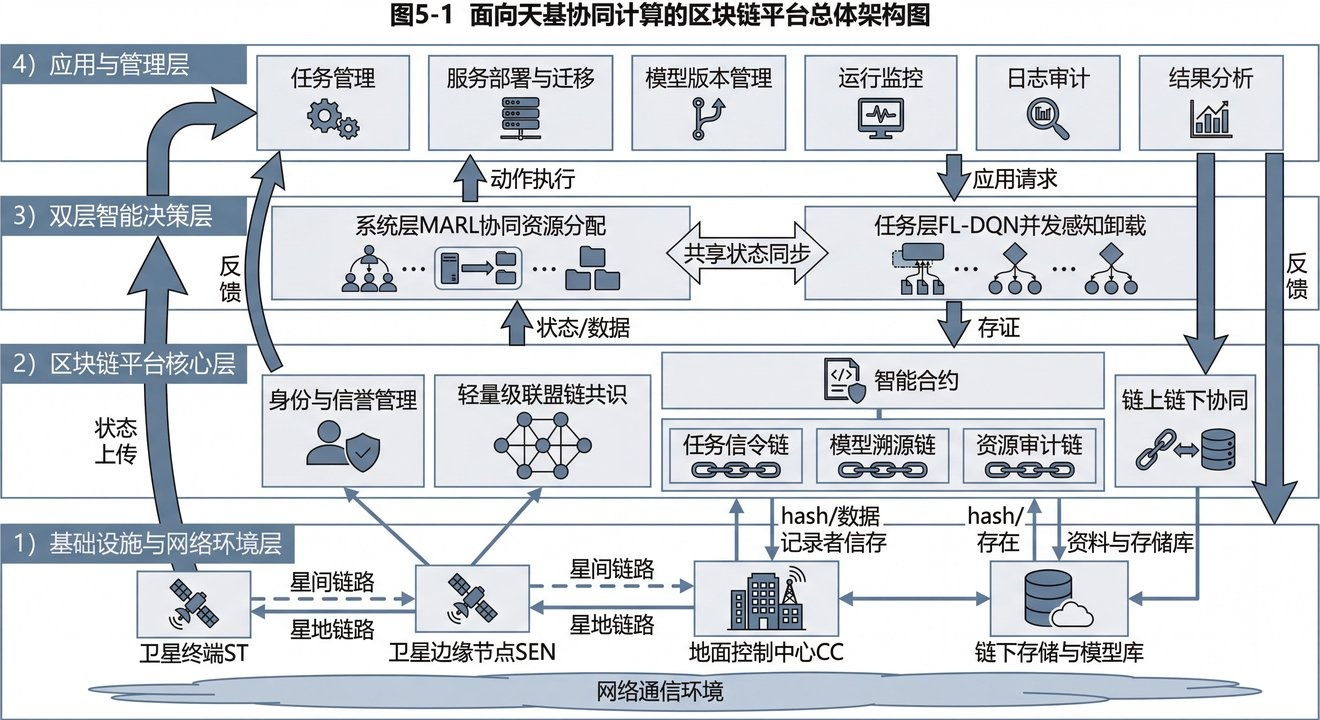
\includegraphics[width=0.96\textwidth]{figures/5-1.jpeg}
  \caption{面向天基协同计算的区块链平台总体架构图}
  \label{fig:platform-arch}
\end{figure}

在网络映射方面，平台将天基协同网络抽象为时变有向图，并据此区分共识维护节点与普通业务节点。定义时刻 $t$ 的天基协同网络为时变有向图
\[\mathcal{G}(t)=({\mathcal{V}},{\mathcal{E}}(t)),\]
其中，节点集合 $\mathcal{V}$ 表示参与天基协同计算与区块链维护的星地节点集合，边集合 $\mathcal{E}(t)$ 表示随时间变化的星间或星地通信连接关系。进一步将节点划分为负责区块打包、共识验证与全局状态定序的共识节点集合 $\mathcal{C}$，以及负责发起任务请求、状态上报和局部决策的普通节点集合 $\mathcal{L}$，满足
\[\mathcal{C}\subseteq \mathcal{V}, \qquad \mathcal{L}=\mathcal{V}\setminus \mathcal{C}.\]

进一步地，为避免平台层建模停留于纯粹的网络拓扑抽象，本文借鉴支撑项目中的天基网络试验任务调度思想，将平台中的任务—资源映射进一步表述为
\[\mathrm{SNEMS}=\{T,R,X,F\}\]
的四元组决策空间。其中，$T$ 表示待调度任务集合，$R$ 表示由平台集、载荷集、窗口集和执行时机构成的资源集合，$X$ 表示任务—资源决策矩阵，$F$ 表示由硬约束与收益函数构成的评价集合。该定义的作用不在于替代第2章的系统模型，而在于为第5章的平台化实现补充"任务如何进入区块链治理框架、资源如何进入系统层动作空间、局部决策如何受全局约束"的统一表达接口。

\textbf{分层链组织与运行接口。}
在平台运行过程中，不同类型的业务事件在频率、时延需求和安全等级方面存在明显差异。结合项目中已有的分层联盟链方案，平台将链结构划分为主链层、子链层和链下设备层。其中，主链负责任务调度、全局状态摘要、日志摘要及关键治理信息维护；子链负责特定区域、特定业务或特定任务类型的数据存证与协同；链下设备层负责原始数据、模型参数和大对象日志的缓存与对象化存储。

从节点角色看，平台可进一步区分为共识节点与非共识节点。主链共识节点负责区块打包、交易校验和全局广播；子链共识节点负责局部数据验证与存证；非共识节点主要承担任务接入、数据采集、状态上报和链下存储等功能。这一划分与项目中的主链—子链—边端设备设计保持一致，有助于在可信性与资源开销之间取得平衡。

进一步地，设平台在时刻 $t$ 的全局状态为 $S^{(t)}$，则在新区块 $B_h$ 经过共识确认后，平台可通过状态转移函数 $\Gamma(\cdot)$ 完成状态更新：
\[S^{(t+1)}=\Gamma\!\left(S^{(t)}, B_h, \Omega_{\text{rules}}\right),\]
其中，$\Omega_{\text{rules}}$ 表示平台治理规则与约束集合，其内部可映射第3章系统层协同策略所给出的全局资源边界、节点信誉约束和任务处理规则。

平台在区块链核心层之上提供统一的状态共享与约束传递接口。系统层输出的资源占用上界、节点可调度集合及链路可用区间，将作为任务层决策的外部约束输入；任务层在执行过程中产生的排队时延、任务成功率、资源消耗和异常事件等结果，则进一步回流至链上状态空间，为后续系统层迭代提供反馈依据。

在应用与管理侧，平台进一步提供任务管理、服务部署与迁移、模型版本管理、运行监控、日志分析、审计查询和策略展示等能力，为前文方法提供可观测、可分析和可配置的统一支撑环境。

\begin{figure}[htbp]
  \centering
  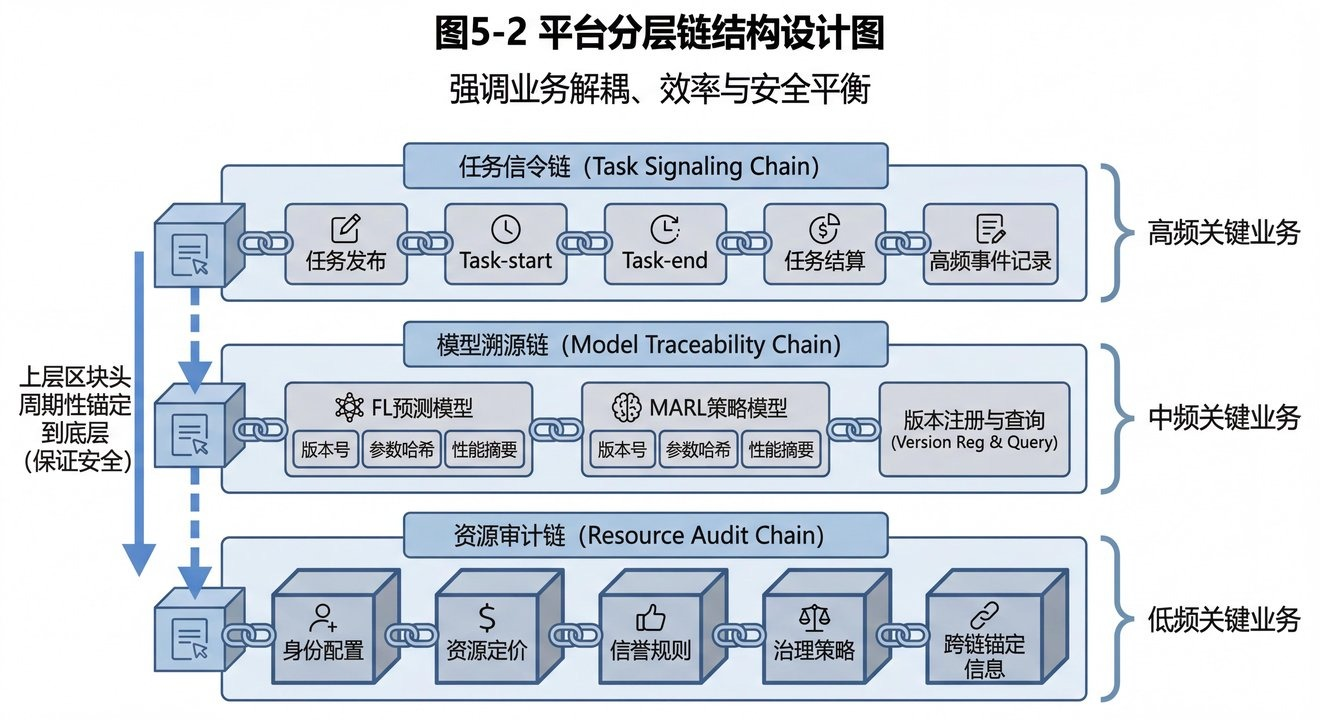
\includegraphics[width=0.92\textwidth]{figures/5-2.jpeg}
  \caption{平台分层链结构设计图}
  \label{fig:chain-arch}
\end{figure}

\section{区块结构、数据流转与存证机制}

\textbf{分层联盟链与链上/链下协同设计。}
传统公有链普遍采用工作量证明等高消耗共识机制，但该类机制难以适应天基网络环境下节点算力受限、能量预算紧张和业务时延敏感的实际约束。对于本文研究场景而言，平台更适合采用许可制联盟链结构，仅允许经过授权的卫星边缘节点、控制节点和少量高可信节点参与账本维护与交易验证，以减少无效竞争开销。

在具体机制选择上，权威证明和委托权益证明是两类较为适合的候选方案。权威证明依赖授权节点轮流出块，适合作为平台初始部署阶段的基础方案；委托权益证明则在保持较高效率的同时，引入代表节点选举机制，可结合节点信誉值、历史贡献度和服务能力动态调整记账节点集合，更适合平台进入稳定运行后的自治演进场景。

\textbf{区块结构与链上/链下协同。}
结合项目中的主链—子链设计，平台继承主链与子链的差异化区块结构。主链区块主要承载任务元数据、跨链摘要、治理规则、资源分配摘要与审计索引；子链区块主要承载业务域内的试验数据摘要、任务状态与局部日志记录。主链更强调调度与治理，子链更强调业务数据存证与局部协同。

在链上/链下协同方面，平台采用"链上保存摘要、链下保存实体对象"的分层管理方式。链上主要保存任务标识、状态摘要、模型版本哈希、审计索引、合约结果和关键治理规则等小体积但高价值的信息；链下则保存任务原始输入、完整模型参数、服务镜像和详细日志等大规模对象。链上记录通过哈希指针与链下对象建立映射关系，当节点需要访问链下数据时，可通过对比其哈希值验证对象的一致性与完整性。

结合项目文件中的分层联盟链与跨链网关设计，链上/链下协同机制还可进一步细化为"子链局部存证 + 主链摘要锚定"的双层存储流程。具体而言，任务执行过程中形成的原始数据、模型参数与详细日志首先保存在链下对象存储或边缘服务集群中，子链仅记录其哈希摘要和过程状态；跨链网关随后将子链摘要提交至主链进行全局锚定。

若记某一业务子链上的区块为 $B_s$，其保存的核心内容可抽象表示为
\[B_s=\{D_{\text{hash}},\, H(B_s^-),\, H(B_s)\},\]
主链在接收跨链网关提交的摘要后，将对应锚定区块记为
\[B_m=\{H(B_s),\, H(B_m^-),\, H(B_m)\}.\]
这一设计能够在不显著增加链上存储压力的前提下，为数据完整性与跨域可验证性提供密码学支撑。

\textbf{数据流转、存证流程与可信执行。}
在数据流转方面，平台沿用项目中"任务基础信息生成与广播—资源与数据信息管理—数据存储与验证—跨链接入与调度管理"的处理链路。具体而言，任务基础信息首先在主链层生成并广播，随后任务需求资源、试验数据和日志信息根据业务类型进入对应子链；大规模原始对象保存在链下，由子链记录摘要并通过跨链网关上传主链锚定。

进一步地，项目中的数据存证流程可为本章平台提供直接的工程实现参考。在数据写入过程中，客户端先向主链发起请求并完成身份与权限校验，随后由跨链网关按照路由转发至对应数据子链；子链完成写入后，将隐私数据哈希、存储位置和过程摘要回传主链存证。在数据读取过程中，主链先完成身份与权限确认，再由跨链网关访问对应子链并返回数据结果与哈希校验信息。由此，项目中的主链—子链—跨链网关—链下对象存储流程，正好为本章平台中的任务状态存证、模型版本锚定和执行日志回写提供了工程模板。

在分布式天基环境下，仅依赖人工配置和静态规则难以保证协同过程的持续稳定运行。为了将任务流转、模型治理和安全约束等关键逻辑由"人为约束"转化为"规则自动执行"，本文在平台中引入智能合约治理机制。任务管理合约用于完成任务注册、参数校验、任务接纳确认、执行开始记录、完成结果写回以及结算与奖惩触发；模型版本管理合约用于登记第4章联邦学习并发开销预测模型与第3章系统层策略模型的版本号、参数哈希、性能摘要和更新时间等内容。

进一步地，考虑到第4章中的联邦学习模型需要在多节点条件下持续演化，平台可将节点信誉值纳入模型聚合过程。即在完成本地训练后，各节点仅提交参数摘要、版本信息及必要的聚合索引，链下完成模型参数交换，链上则记录版本登记与合法性校验结果；对于信誉值持续偏低或存在异常行为的节点，其提交的聚合权重可被削弱或拒绝，从而增强模型治理的可靠性。

\section{双层智能方法的平台映射与运行闭环}

\textbf{系统层与任务层方法的平台映射。}
第3章提出的基于区块链与多智能体强化学习的系统层协同资源分配方法，主要面向全局尺度下的资源竞争与协同优化问题。在平台化实现中，该方法被映射为双层智能决策层中的系统层控制模块，其核心职责不再是单纯输出离线策略，而是持续接收链上共享状态并对全局资源边界进行动态更新。

具体而言，平台通过区块链核心层维护节点负载摘要、可用算力信息、链路质量指标、历史信誉状态以及任务分布统计结果等公共环境变量。系统层智能体在此基础上依据马尔可夫博弈框架进行策略更新，并形成资源分配建议、节点协同关系和服务能力边界等结果。这些结果并不直接替代任务层决策，而是以资源约束、候选集优先级和协同调度边界的形式向下传递。

在任务层，第4章提出的并发感知卸载方法被映射为局部实时决策模块，其输入由任务属性、本地节点状态、候选节点共享状态、系统层约束边界以及联邦学习模型预测结果共同构成。联邦学习预测模型的版本信息和参数摘要由模型版本管理合约统一维护，任务层节点在调用模型前可通过链上查询确认其版本合法性，并对模型参数进行哈希校验，从而保证预测输入来源可信。

\textbf{状态—动作—存证—反馈闭环。}
为了更清晰地描述平台中双层智能决策的运行逻辑，本文将平台核心流程抽象为"状态—动作—存证—反馈"闭环机制。设平台在时刻 $t$ 的联合状态表示为
\[S(t)=\{S_{\text{sys}}(t),\, S_{\text{task}}(t),\, S_{\text{chain}}(t)\},\]
其中，$S_{\text{sys}}(t)$ 表示系统层公共状态，$S_{\text{task}}(t)$ 表示任务层局部状态，$S_{\text{chain}}(t)$ 表示链上共享状态。

系统层根据联合状态生成资源协同动作 $a_{\text{sys}}(t)$，任务层结合局部状态与系统层约束生成卸载动作 $a_{\text{task}}(t)$。因此，平台在时刻 $t$ 的联合动作可表示为
\[A(t)=\{a_{\text{sys}}(t),\, a_{\text{task}}(t)\}.\]

在动作执行后，平台通过智能合约将关键行为记录为链上事件集合
\[E(t)=\{e_{\text{start}}(t),\, e_{\text{end}}(t),\, e_{\text{model}}(t),\, e_{\text{audit}}(t)\}.\]

在反馈阶段，任务执行所产生的时延、能耗、资源占用变化和任务完成质量等结果被汇聚为反馈向量 $F(t)$，并用于更新下一时刻的平台状态，即
\[S(t+1)=\Phi\!\left(S(t),A(t),E(t),F(t)\right).\]

\begin{figure}[htbp]
  \centering
  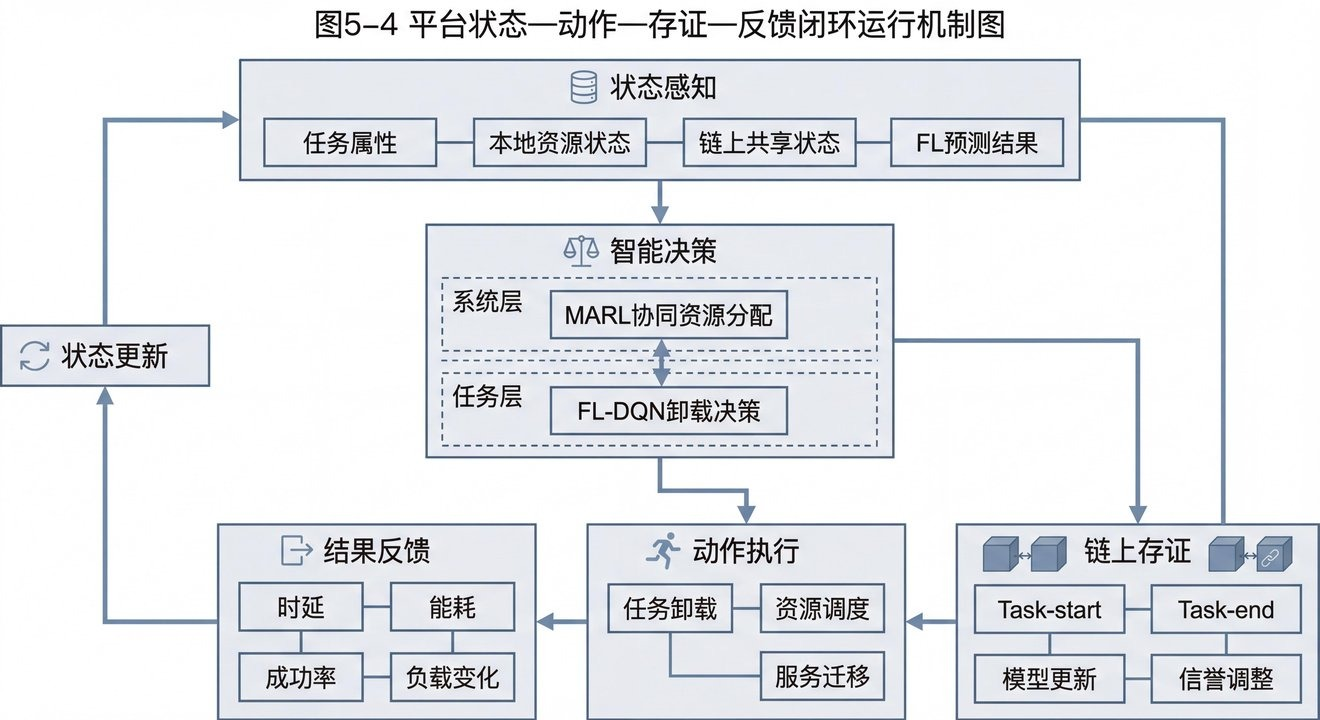
\includegraphics[width=0.92\textwidth]{figures/5-4.jpeg}
  \caption{平台状态—动作—存证—反馈闭环运行机制图}
  \label{fig:closed-loop}
\end{figure}

\textbf{资源审计、身份控制与信誉评估。}
第3章提出的系统层多智能体强化学习方法输出的是全局资源协同结果，而第4章任务层方法则面向单任务到达瞬间做出局部动作选择。为了避免两层决策彼此割裂，平台需要建立从系统层到任务层的约束传递机制。为此，平台可将系统层输出的协同动作表示为 $A_{\text{sys}}$，并进一步映射为面向任务层的局部约束集合 $C_{\text{limit}}$。当单任务到达并触发任务层深度强化学习决策时，其可行动作空间可表示为
\[A'_{\text{task}}=A_{\text{task}}\cap C_{\text{limit}}.\]

在身份认证方面，平台采用联盟链白名单准入机制，仅允许经过授权的节点参与网络；并通过数据访问授权与合约调用授权，限制不同角色对任务信息、试验数据、模型版本与治理合约的操作权限。该部分直接继承了项目中已有的身份管理与访问控制思路。

在资源审计与信誉评估方面，平台持续记录节点的资源声明、任务接纳情况、实际执行结果和历史服务质量，并结合审计规则对其一致性进行检查。设节点 $i$ 在时间窗 $\tau$ 内的信誉值为 $R_i(\tau)$，则其更新可表示为
\[R_i(\tau)=\alpha R_i(\tau-1)+(1-\alpha)\sum_{k\in T_i} I(\text{link}_k)\,\omega_k\,\varphi(k),\]
其中，$\alpha\in(0,1)$ 为历史遗忘因子，$\omega_k$ 为任务重要度权重，$\varphi(k)$ 表示任务 $k$ 的执行评价项，$I(\text{link}_k)$ 为链路状态感知因子，用于刻画任务执行期间对应星间或星地链路是否处于可见且可通信状态。

\section{平台运行流程、工程分析与本章小结}

\textbf{平台运行流程。}
为进一步展示平台的数据流转机制，本节结合灾害应急多星协同计算场景，对双层智能方法在平台中的运行逻辑进行说明。系统初始阶段，各卫星节点同步包含全局负载摘要与模型版本哈希的最新区块头，并结合本地缓存完成运行状态初始化。当高密度遥感图像识别任务在某一低轨卫星节点产生后，任务层首先提取局部状态，并从链下模型库获取当前有效模型参数，通过模型版本管理合约完成哈希一致性校验。在模型合法性得到确认后，任务层深度强化学习模块输出具体卸载动作。

随后，任务请求进入平台合约处理流程。跨层约束机制将依据系统层资源协同结果判断目标节点是否仍处于允许接纳任务的资源边界之内。若满足约束条件，则平台生成任务开始事件并记录相应状态；若不满足，则任务需重新选择候选节点或回退至本地执行。待任务执行结束后，系统将时延、能耗和完成质量等结果封装为反馈信息写回平台，并同步完成链上存证、信誉结算和样本沉淀。

模型更新与版本治理过程中，各节点基于本地任务样本开展联邦训练，聚合后的新模型由版本管理合约登记其版本号、参数哈希与性能摘要。平台还可在检测到局部区域出现任务热点、节点拥塞或服务失衡时，触发服务部署与迁移流程，以保持系统能力分布的动态均衡。

\textbf{平台项目对前文方法的支撑作用。}
从全文结构看，本章引入平台项目的目的，在于把前文分散于模型、算法和决策层的研究内容串联起来。第2章给出了天基协同计算的系统模型与状态约束，第3章提出了基于区块链与多智能体强化学习的系统层协同资源分配方法，第4章提出了基于联邦学习与深度强化学习的任务层并发感知卸载方法；而本章则依托项目中已完成的分层联盟链、主链—子链区块结构、跨链网关、数据流转与存证流程、以及身份与访问控制等设计，为这些方法提供统一的工程承载环境。

\textbf{工程可行性分析。}
为进一步验证本文所设计区块链平台架构在天基动态环境下的可行性，本文结合 STK 生成星座轨道与可见性关系，并利用 NS-3 构建网络层通信仿真环境。仿真重点关注平台在共识开销、存储增长和异常节点隔离等方面的运行特性，以检验平台对前文双层智能方法的承载能力。

评估指标主要包括确认时延、存储开销增长以及信誉驱动的异常节点隔离效果等。通过上述配置，可以从"吞吐与时延""存储可持续性""异常治理能力"三个维度对平台工程适应性进行考察。综合结果表明，平台在吞吐能力、确认时延、存储控制和异常治理等方面均表现出较好的工程适应性。

\textbf{本章小结。}
综合上述分析可以看出，本章所设计的平台并非对前文算法的简单附属说明，而是依托已完成的平台项目，将系统建模、系统层协同优化与任务层实时决策统一到一个可运行、可验证、可审计的工程框架中。其中，项目中已有的分层联盟链、主链—子链区块结构、跨链网关、数据流转与存证流程、以及身份与访问控制等设计，为平台的可信状态同步、任务行为存证、模型版本治理和执行反馈闭环提供了直接支撑；而第3章和第4章提出的双层智能方法，则在这一平台上完成了从算法层到系统层的落地映射。由此，本文实现了从系统模型、算法设计到平台实现的研究链条闭合，也使第五章真正承担起"用平台项目把前几章串起来"的作用。